% Section content template for individual Educative lessons
% This file contains the actual content for a specific section
% Generated from Educative API section content

% Section: System Design: Instagram
% Section ID: 5206574926921728
% Section Slug: system-design-instagram
% Generated: 2025-12-08T13:38:54.055953

\subsection{What is Instagram?}\label{VhE_Jw-NMeT_bcqY8NMcU}
\\
\textbf{Instagram} is a free social networking application that allows users to upload photos and short videos. Users can add a caption for each post and utilize hashtags or location-based geotags to index them and make them searchable within the application. Posts appear in a user's followers' newsfeeds, and content tagged with hashtags or geotags can be accessed by the broader public, helping users reach a wider audience. Users can also choose to make their profile private, which limits access to those who have chosen to follow them.

\begin{figure}[htbp]
 \centering
 
\includegraphics[width=0.15\textwidth]{Images/chapter_33/section_5206574926921728/6312945401069568.png}
 
\end{figure}

\begin{quote}
\textbf{Note:} As Instagram\textquotesingle s user base grows globally, the demand for resources such as servers, databases, and content delivery networks (CDNs) also increases. Instagram must continously optimize its backend architecture to meet the increasing demands of millions of daily active users. Efficiently managing user growth, predicting future resouce requirements, and ensuring scalability are essential for handling the massive volumes of real-time, user generated content.
\end{quote}
\\
The expansion in the number of users requires more resources (servers, databases, and so on) over time. Knowing the users' growth rate helps us predict the resources to scale our system accordingly. The following illustration shows the Instagram user base in different countries as of January 2022 (source: Statista).

\begin{figure}[htbp]
 \centering
 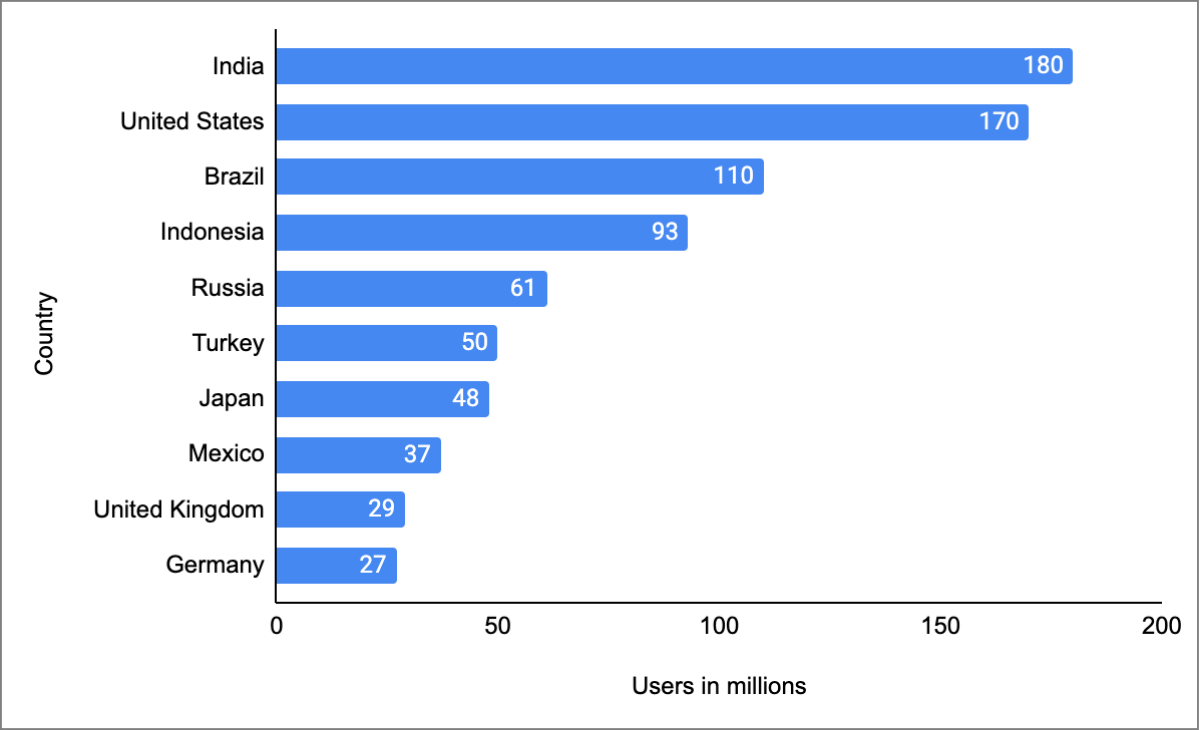
\includegraphics[width=0.5\textwidth]{Images/chapter_33/section_5206574926921728/5945006909292544.png}
 \caption{Countries with the most Instagram users}
\end{figure}

\textbf{Did you know?}
\\
Instagram\textquotesingle s seamless user experience---instant notifications, personalized feeds, and high availability is driven by a powerful system design using Redis, Cassandra, and advanced file storage. Explore how these technologies power the social media giant and inspire top engineering interview questions!

\subsection{How will we design Instagram?}\label{5WDafaiehoFLE6a-neYQh}
\\
This section is designed for aspiring software engineers or those preparing for system design interviews. We have divided the design of Instagram into four lessons:

\begin{enumerate}
\item
\protect\phantomsection\label{sOTQcbKAD_xmOELebf2tO}
\href{https://www.educative.io/courses/grokking-the-system-design-interview/requirements-of-instagrams-design}{\textbf{Requirements}}: This lesson will put forth the functional and nonfunctional requirements of Instagram. It will also estimate the resources required to achieve these requirements.
\item
\protect\phantomsection\label{vk-PYuxnq8896Ob-CxuAs}
\href{https://www.educative.io/courses/grokking-the-system-design-interview/design-of-instagram}{\textbf{Design}}: This lesson will explain the workflow and usage of each component, its high-level design, API design and database schema.
\item
\protect\phantomsection\label{DAM3KoX3_EaJBtVHE30Lm}
\href{https://www.educative.io/courses/grokking-the-system-design-interview/detailed-design-of-instagram}{\textbf{Detailed design}}: In this lesson, we'll explore the components of our Instagram design in detail, discuss various approaches to generating timelines, and evaluate our proposed design.
\item
\protect\phantomsection\label{EgC5bJ0jq2eCEzzxlX79p}
\href{https://www.educative.io/courses/grokking-the-system-design-interview/quiz-on-instagrams-design}{\textbf{Quiz}}: This lesson will test our understanding of the Instagram design.
\end{enumerate}

\begin{itemize}
\item
How can Instagram handle feed generation and messaging to deliver personalized user feeds, integrate notifications, and ensure reliable storage and retrieval of feed data for optimal photo-sharing functionality?
\item
How do load balancers, rate limiters, and Kafka help ensure Instgram\textquotesingle s performance during peak activity, streamlining messaging and handling millions of user requests with low latency and optimal user experience?
\item
Why is selecting the right data store (NoSQL vs. relational databases) crucial for managing user data, feed data, and high volumes of requests while maintaining scalability and reliability?
\item
What considerations must Instagram address when implementing file and object storage (e.g., Amazon S3), and how do sharding and replication impact large-scale photo-sharing?
\end{itemize}
\\
Let's start by understanding the requirements for designing our Instagram system, using practical insights on distributed systems and API optimization. In the next lesson, we will provide resource estimations.

% End of section content